\documentclass[11pt]{article}

\usepackage{latexsym}
\usepackage{amssymb}
\usepackage{amsthm}
\usepackage{enumerate}
\usepackage{amsmath}
\usepackage{cancel}
\usepackage{graphicx}
\numberwithin{equation}{section}
\numberwithin{figure}{section}
\numberwithin{table}{section}

\setlength{\evensidemargin}{.25in}
\setlength{\oddsidemargin}{-.25in}
\setlength{\topmargin}{-.75in}
\setlength{\textwidth}{6.5in}
\setlength{\textheight}{9.5in}
\newcommand{\due}{February 18th, 2010}
\newcommand{\HWnum}{3}
\newcommand{\grad}{\bold\nabla}
\newcommand{\vecE}{\vec{E}}
\newcommand{\scrptR}{\vec{\mathfrak{R}}}
\newcommand{\kapa}{\frac{1}{4\pi\epsilon_0}}
\newcommand{\unit}[1]{\ensuremath{\, \mathrm{#1}}}

\begin{document}
\begin{titlepage}
\setlength{\topmargin}{1.5in}
\begin{center}
\Huge{Physics 3320} \\
\LARGE{Principles of Electricity and Magnetism II} \\
\Large{Professor Ana Maria Rey} \\[1cm]

\huge{Homework \#\HWnum}\\[0.5cm]

\large{Joe Becker} \\
\large{SID: 810-07-1484} \\
\large{\due} 

\end{center}

\end{titlepage}



\section{Introduction}
Often during an experiment the signal we are trying to measure has very small voltage. In these cases we want to amplify the signal. To do the we use an operational amplifier (op-amp for short). 

In this experiment we will demonstrate the properties of common op-amps both inverting and non-inverting and their behaviour under differing frequencies.

\section{Theory}
The most basic op-amps have a transfer function defined as
\begin{equation}
A\equiv\frac{V_{out}}{V^+_{in}-V^-_{in}}
\label{EquA}
\end{equation}
Where $V^+_{in}$ is the voltage input into the positive terminal and $V^-_{in}$ is the voltage input into the negative terminal. We see that the output voltage scales to the difference of the two input voltages. This is why we often call $A$ the gain of the op-amp. But the op-amp by itself does not have very good stability despite the high gain. To compensate for this we often incorporate a feedback loop into the circuit. For this experiment we test two different negative feedback loops, an inverting and non-inverting amplifier. Note that a negative feedback loop is when $V_{out}$ is feed into the negative input. 

\subsection{Non-Inverting Amplifier}
A basic non inverting amplifier as seen in figure \ref{FigNonInvAmp}
\begin{figure}[h]
\centering
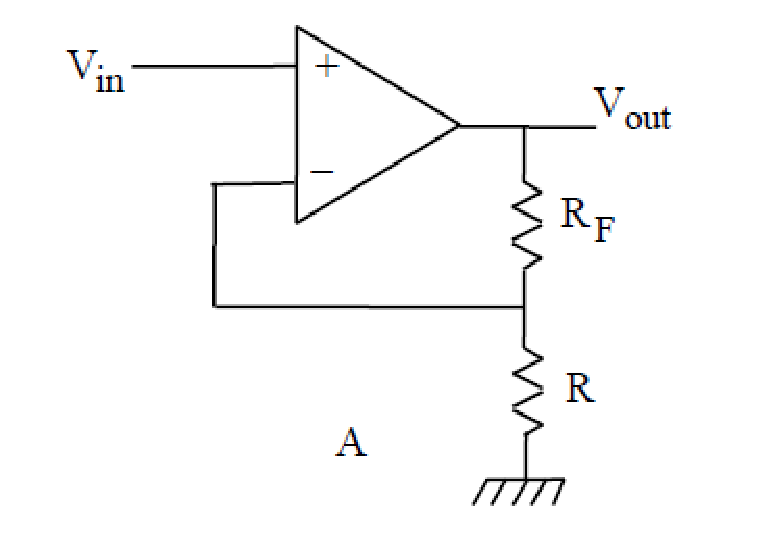
\includegraphics[scale=0.60]{FigNonInvAmp.eps}
\caption{\textit{A simple non-inverting amplifier}}
\label{FigNonInvAmp}
\end{figure}
We see that the gain of this circuit from equation \ref{EquA} is given by
$$V_{out} = A(V_{in}-BV_{out})$$
where $B$ is derived from the voltage divider ratio in the feedback loop and is given by
\begin{equation}
B\equiv\frac{R}{R+R_F}
\label{BVoltDiv}
\end{equation}
so we can see that the gain $G=V_{in}/V_{out}$ is given by 
\begin{equation}
G = \frac{A}{1+AB}
\label{NonInvGain}
\end{equation}
Now if we assume that $A$ is very large we can approximate $G$ as
$$G = 1+\frac{R_F}{R}$$
Now if we vary the frequency of the input voltage we see that the open loop gain $A$ will vary as
\begin{equation}
A = \frac{A_0}{1+i\dfrac{f}{f_0}}
\label{AFreq}
\end{equation}
where $A_0$ is the DC gain and $f_0$ is the $3$dB frequency. Though we usually are given the value $f_T$ which is the frequency where the magnitude of the open loop gain $A$ is one. And we find $f_0$ using
\begin{equation}
f_T = A_0f_0
\label{fTEqu}
\end{equation}
Also we can find the closed loop gain $g$ frequency dependence by substituting equation \ref{AFreq} into equation \ref{NonInvGain} to get
\begin{equation}
G = \frac{G_0}{1+i\dfrac{f}{f_B}}
\label{FreqGain}
\end{equation}
Where $f_B$ is the $3$dB bandwidth and it is given by
\begin{equation}
f_B =  f_0(1+A_0B)
\label{FreqB}
\end{equation}
and $G_0$ is the DC closed loop gain which is the gain for frequencies below $f_B$. We can find $G_0$ from
\begin{equation}
G_0 = \frac{A_0}{1+A_0B}
\label{G0NonInv}
\end{equation}
We can also relate $f_B$ and $G_0$ to $f_T$ using the gain-bandwidth product which is
\begin{equation}
G_0f_B = f_T
\label{GainBandProd}
\end{equation}

\subsection{Inverting Amplifier}
A simple inverting amplifier is shown in figure \ref{FigInvAmp}. Note that the positive terminal is grounded, so the op-amp is going to try and keep the negative terminal at ground too. 
\begin{figure}[h]
\centering
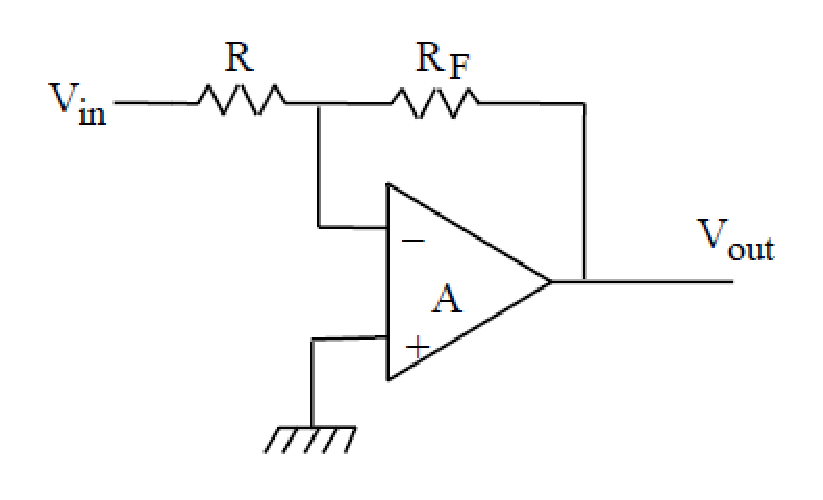
\includegraphics[scale=0.60]{FigInvAmp.eps}
\caption{\textit{A simple inverting amplifier}}
\label{FigInvAmp}
\end{figure}
This coupled with the fact that the inputs draw no current lead to us seeing that
$$\frac{V_{in}}{R} = -\frac{V_{out}}{R_F}$$
So we can say that the dc closed loop gain $G_0$ is given by
$$G_0 = \frac{V_{out}}{V_{in}}=-\frac{R_F}{R}$$
But these are only true under the assumption that $A\rightarrow\infty$ if we need to take into account a finite $A$ we can see that
$$V^-_{in} = V_{in}+B(V_{out}-V_{in})$$
from equation \ref{EquA}. And we can see that the negative terminal's input voltage is given by $V_{in}^- = -V_{out}/A$ so we can say that the gain of the inverting amplifier is 
\begin{equation}
G = \frac{-A(1-B)}{1+AB}
\label{GainInvAmp}
\end{equation}
Now the frequency dependence for the inverting case is the same as the non-inverting case. So to find $A$ we still can use equation \ref{AFreq} and equation \ref{fTEqu} will also give us $f_0$. Also we note that equations \ref{FreqB} and \ref{FreqGain} are both valid for this circuit. But for low enough frequencies (below $f_B$) the DC closed loop gain $G_0$ is different from equation \ref{G0NonInv} and is given by
\begin{equation}
G_0 = -\frac{A_0(1-B)}{1+A_0B}
\label{G0InvAmp}
\end{equation}
We also note that the gain-bandwidth product is different for the inverting case it is as follows
\begin{equation}
G_0f_B = -f_T(1-B)
\label{InvGainBand}
\end{equation}

The input impedance of an op-amp in the inverting case is given by the equation 
\begin{equation}
Z_{in} = R+\frac{R_F}{1+A}
\label{InputImp}
\end{equation}

\section{Experiment}
To begin the experiment we set up the function generator, DC power supply, and the oscilloscope. We split the output of the function generator to the first input of the oscilloscope and into the circuit. The output voltage from the circuit was connected to the second channel of the oscilloscope. We used the power supply to power the op-amp. 

\subsection{Voltage Follower} 
First we made the voltage follower circuit show in figure \ref{FigVoltFollow}

\begin{figure}[h]
\centering
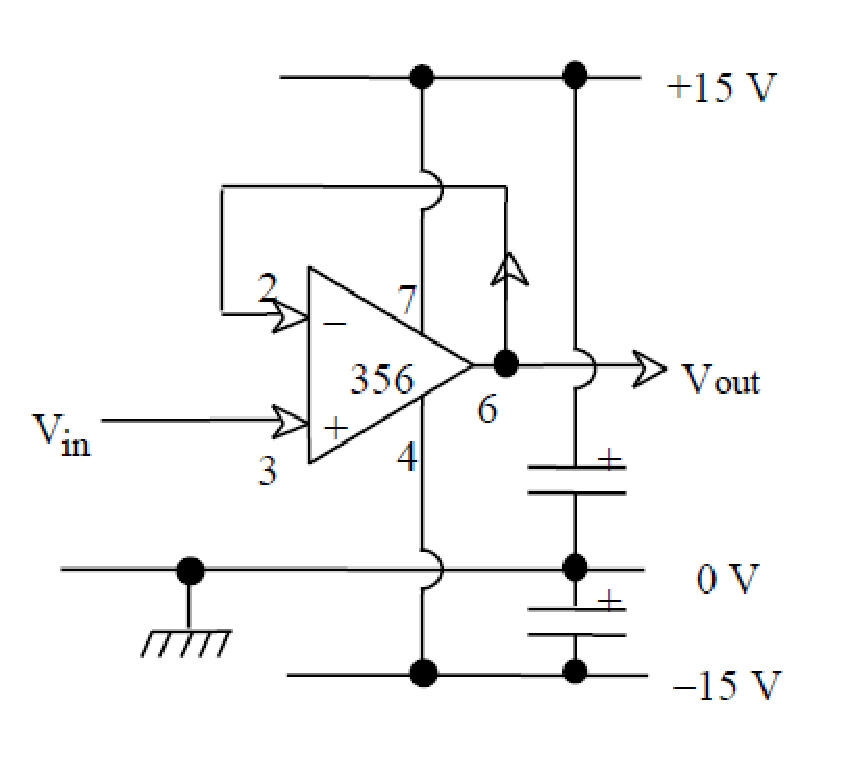
\includegraphics[scale=0.60]{FigVoltFollow.eps}
\caption{\textit{The schematic for the voltage follower circuit}}
\label{FigVoltFollow}
\end{figure}
Once the circuit was constructed we inputed $+15\unit{V}$ into $V_{in}$ to find the saturation voltage. That is the maximum voltage we output. We measured the output voltage using the oscilloscope's cursors and found that $V_{sat} = 13.4\unit{V}$. The data sheet for the LF356 op-amp said that $V_{sat} = \pm13\unit{V}$ so our measured result agrees with what we expect.

Next we changed the input voltage from $+15\unit{V}$ to a sine wave with $1\unit{V\ PP}$ with a frequency of $1.00\unit{kHz}$. Next we used the oscilloscope's cursor to measure $V_{in}$ and $V_{out}$ to find the gain for the voltage follower. We found that $V_{in} = 1.00\unit{V\ PP}$ and $V_{out} = 1.01\unit{V\ PP}$. So we see $G_0 = 1.01$ and we expect a voltage follower to have a gain of $1$ so we see that our measured result agrees with the predicted.

Next we wanted to find $f_B$. So to find $f_B$ we need to find the point where
$$\frac{V_{out}}{V_{in}} = \frac{1}{\sqrt{2}}$$
and we already measured $V_{in}$ as $1.00\unit{V\ PP}$ so we adjusted the frequency until we found $V_{out} = 0.707\unit{V\ PP}$. To do this we increased the frequency on the function generator. We found that the frequency at which the output voltage dropped $3$dB was $f_B = 12.18\unit{MHz}$. Next we measured the change in the gain at different orders of $f_B$. The data we collected is in table \ref{1partc}. This data is plotted in a Bode Plot (figure \ref{PlotVoltFollow}).

\begin{table}[h]
\centering
\begin{tabular}{lccccc}
		&Frequency		&$V_{in}$	&$V_{out}$		&Gain ($G_0$)	&Gain dB\\
\hline
$10^{-5}f_B$	&$121.8\unit{Hz}$	&$1.02\unit{V}$	&$1.01\unit{V}$		&$0.99$	&$-0.087$\\
$10^{-4}f_B$	&$1.218\unit{kHz}$	&$1.02\unit{V}$	&$1.01\unit{V}$		&$0.99$	&$-0.087$\\
$10^{-3}f_B$	&$12.18\unit{kHz}$	&$1.01\unit{V}$	&$1.01\unit{V}$		&$1.00$	&$0.00$\\
$10^{-2}f_B$	&$121.8\unit{kHz}$	&$1.01\unit{V}$	&$1.01\unit{V}$		&$1.00$	&$0.00$\\
$10^{-1}f_B$	&$1.218\unit{MHz}$	&$0.996\unit{V}$&$0.980\unit{V}$	&$0.984$	&$-0.14$\\
$f_B$		&$12.18\unit{MHz}$	&$0.836\unit{V}$&$0.708\unit{V}$	&$0.847$	&$-0.14$\\
\end{tabular}
\caption{\textit{Change in gain at changing orders of $f_B$. Note we measured $V_{in}$ and $V_{out}$ and used the relation $G_0 = V_{out}/V_{in}$ to find the gain.}}
\label{1partc}
\end{table}

\begin{figure}[h]
\centering
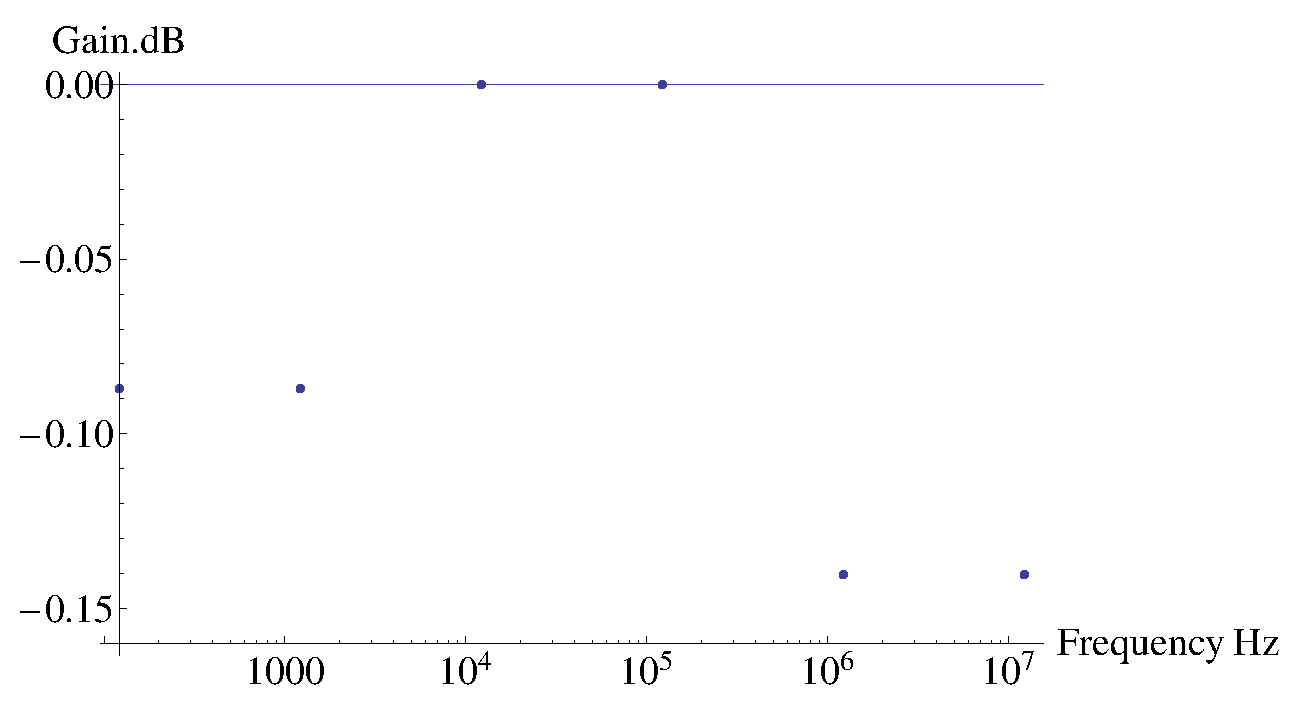
\includegraphics[scale=0.60]{PlotVoltFollow.eps}
\caption{\textit{Bode Plot of the data in table \ref{1partc}. Note that the line is the expected gain in dB ($G_0=0.00$)}}
\label{PlotVoltFollow}
\end{figure}

\subsection{100 Non-inverting Amplifier} 
First we made the circuit described in the schematic in figure \ref{FigNonInvAmpSchem}

\begin{figure}[h]
\centering
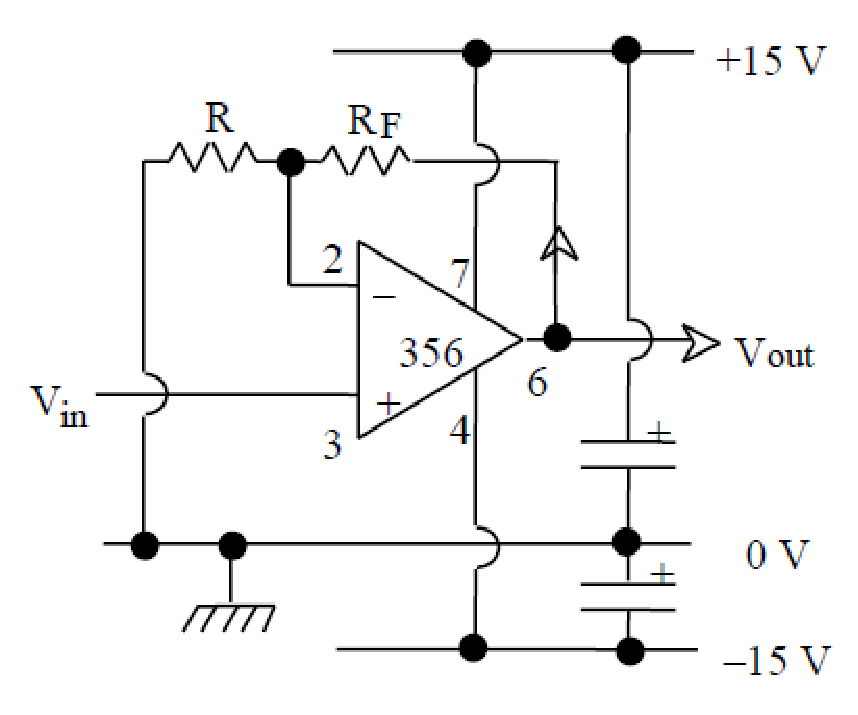
\includegraphics[scale=0.60]{FigNonInvAmpSchem.eps}
\caption{\textit{The schematic for the Gain=100 non-inverting amplifier circuit}}
\label{FigNonInvAmpSchem}
\end{figure}
where $R_F=9.92\unit{k\Omega}$ and $R=99.0\unit{\Omega}$. We then sent a sine wave input voltage with an amplitude of $100\unit{mV\ PP}$ and a frequency of $1.00\unit{kHz}$. We then used the cursors on the oscilloscope to find the input and out. We found that $V_{in}=103\unit{mV}$ and $V_{out}=10.1\unit{V}$. So we measured the closed loop gain $G_0$ as $98.1$. We calculated $G_0$ from equation \ref{G0NonInv} and found that we expected $G_0 = 101$. Note that we used values found in the LF356 op-amp manual for $A_0$ where $A_0=2\times10^{5}$ and we calculated $B$ from equation \ref{BVoltDiv} where $R_F=9.92\unit{k\Omega}$ and $R=99.0\unit{\Omega}$. So we see that our measured and expected result are in agreement.

Next we found $f_B$ for the non-inverting amplifier. To do this we want to find the frequency where the output voltage is $1/\sqrt{2}$ of the output voltage at $1\unit{kHz}$. We measured $V_{out}$ at $1\unit{kHz}$ as $10.1\unit{V}$ so we adjusted the frequency until we reached a voltage of $7.14\unit{V}$. So we found $f_B = 50.3\unit{kHz}$. We can find our expected value of $f_B$ from equation \ref{GainBandProd} where we use $G_0$ we measured as $98.1$ and $f_T$ is given by the LF356 op-amp manual as $f_T = 5\unit{MHz}$. So we calculated $f_B = 51.0\unit{kHz}$. Note that this is congruent with our measured value. 

Next we found the change in gain with respect to different orders of $f_B$ and put the date in table \ref{2parta}.

\begin{table}[h]
\centering
\begin{tabular}{lccccc}
		&Frequency		&$V_{in}$	&$V_{out}$		&Gain ($G_0$)	&Gain dB\\
\hline
$10^{-3}f_B$	&$50.3\unit{Hz}$	&$0.103\unit{V}$	&$10.3\unit{V}$		&$100$	&$40.0$\\
$10^{-2}f_B$	&$503\unit{Hz}$		&$0.103\unit{V}$	&$10.3\unit{V}$		&$100$	&$40.0$\\
$10^{-1}f_B$	&$5.03\unit{kHz}$	&$0.102\unit{V}$	&$10.2\unit{V}$		&$100$	&$40.0$\\
$f_B$		&$50.3\unit{kHz}$	&$0.102\unit{V}$	&$7.28\unit{V}$		&$71.4$	&$37.1$\\
$10^{1}f_B$	&$503\unit{kHz}$	&$0.103\unit{V}$	&$1.05\unit{V}$		&$10.2$	&$20.2$\\
$10^{2}f_B$	&$5.03\unit{MHz}$	&$0.126\unit{V}$	&$0.097\unit{V}$	&$0.77$	&$-2.27$
\end{tabular}
\caption{\textit{Change in gain at changing orders of $f_B$ of the non-inverting amplifier. Note we measured $V_{in}$ and $V_{out}$ and used the relation $G_0 = V_{out}/V_{in}$ to find the gain.}}
\label{2parta}
\end{table}
We plotted the data from table \ref{2parta} in a Bode plot (see figure \ref{PlotNonInvAmp}).

\begin{figure}[h]
\centering
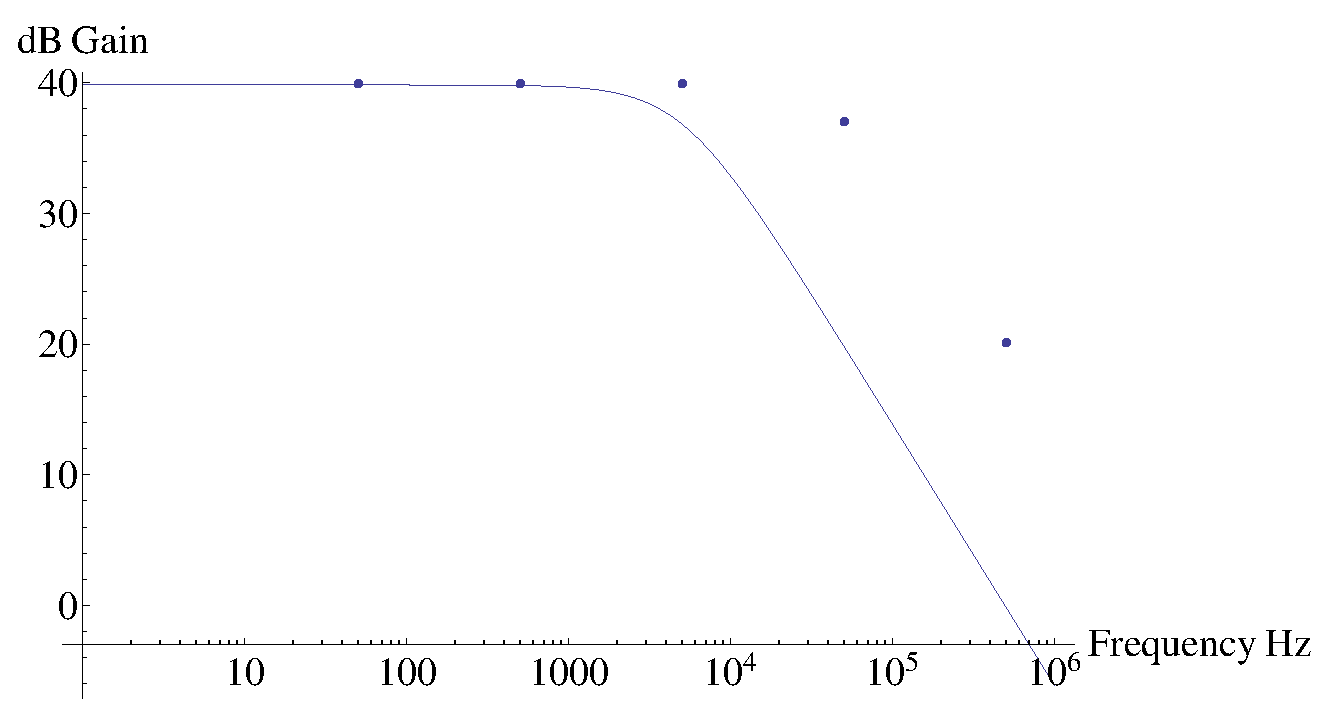
\includegraphics[scale=0.60]{PlotNonInvAmp.eps}
\caption{\textit{Bode Plot of the data in table \ref{2parta}. Note that the line is the theoretical gain given by equation \ref{FreqGain}}}
\label{PlotNonInvAmp}
\end{figure}

Note that we assume the input impedance of this circuit is very high. So we put a resistor $R_s=0.992\unit{M\Omega}$ in series with the input voltage to see if there was a change in the signal. We saw no change in the circuit so we confirmed that the input impedance is high.

\subsection{Inverting Amplifier} 
First we made a circuit like that in figure \ref{FigInvAmp} where $R_F=2.66\unit{k\Omega}$ and $R=267.9\unit{\Omega}$. Then we sent an sinusoidal input voltage with an amplitude of $100\unit{mV}$. We varied the frequency by powers of ten and measured the change in the gain $G_0$. This data is in table \ref{3parta}

\begin{table}[h]
\centering
\begin{tabular}{lccccc}
&Frequency		&$V_{in}$	&$V_{out}$		&Gain ($G_0$)	&Gain dB\\
\hline
&$100\unit{Hz}$		&$86.4\unit{mV}$&$-848\unit{mV}$	&$-9.81$	&$19.8$\\
&$1.00\unit{kHz}$	&$85.6\unit{V}$	&$-852\unit{mV}$	&$-9.95$	&$20.0$\\
&$10.0\unit{kHz}$	&$86.4\unit{V}$	&$-860\unit{mV}$	&$-9.95$	&$20.0$\\
&$100\unit{kHz}$	&$86.4\unit{V}$	&$-836\unit{mV}$	&$-9.68$	&$19.7$\\
&$1.00\unit{MHz}$	&$98.8\unit{V}$	&$-428\unit{mV}$	&$-4.33$	&$12.7$\\
&$10.0\unit{MHz}$	&$86.0\unit{V}$	&$-62.0\unit{mV}$	&$-0.72$	&$-2.85$
\end{tabular}
\caption{\textit{Change in gain at changing orders of $f_B$ of the inverting amplifier. Note we measured $V_{in}$ and $V_{out}$ and used the relation $G_0 = V_{out}/V_{in}$ to find the gain.}}
\label{3parta}
\end{table}
We plotted the data in table \ref{3parta} in a Bode plot see figure \ref{PlotInvAmp}

\begin{figure}[h]
\centering
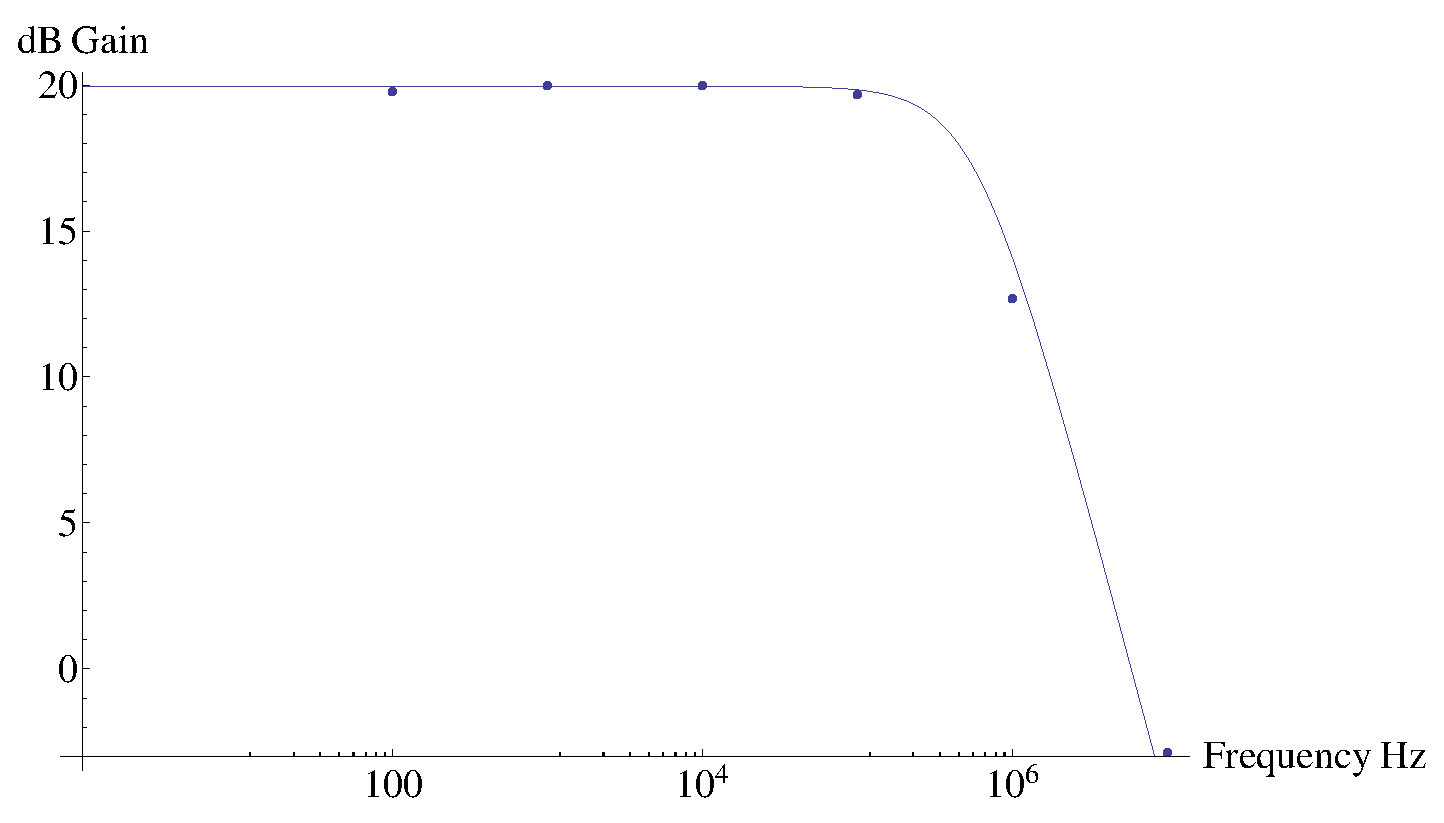
\includegraphics[scale=0.60]{PlotInvAmp.eps}
\caption{\textit{Bode Plot of the data in table \ref{3parta}. Note that the line is the theoretical gain given by equation \ref{FreqGain}}}
\label{PlotInvAmp}
\end{figure}

Next we found $f_B$ to do this we needed to find the point where the voltage dropped to $1/\sqrt{2}$ of the voltage out at $1\unit{kHz}$ we calculated this point to be $602\unit{mV}$. So we increased the voltage until we found $V_{out}=602\unit{mV}$ this was at $f_B = 592.0\unit{kHz}$. Using equation \ref{InvGainBand} we calculated $f_B=457.9\unit{kHz}$. Note that these values do not agree all that well, this is due in part to the fact that we are not at the exact $3$dB point.

Finally we measured the input impedance of the inverting amplifier by connection a variable resistor in series with the input resistor. This created a voltage divider where one resistor is the impedance of the circuit and the other resistor is the potentiometer. We know that the two resistances are equal when the voltage out is half of the voltage in, so we adjusted the potentiometer until our $V_{out}=\frac{1}{2}V_{in}$ and then measured the resistance of the potentiometer as $Z_{in} = 282.4\unit{\Omega}$. Using equation \ref{InputImp} we calculated the input impedance to be $Z_{in} = 281.1\unit{\Omega}$. We see that our measured and expected results are in agreement.

\section{Conclusion}
In this lab we demonstrated the basic properties of an operational amplifier with feedback loops. We saw that high frequencies the gains dropped and the circuits started to behave like RC circuits. We also saw how the feed back resistance effected the gain.
\end{document}

